\chapter{
  Event Simulation and Reconstruction
 }\label{ch_reco}

The proton-proton collision at the \gls{LHC} produces a shower of particles. Before
the event information can be easily used in an analysis, the data collected goes
through an iterative process of reconstruction of particles produced in the collision.
\gls{CMS} uses a \gls{PF} algorithm to reconstruct 4-vectors of muons, electrons,
photons, hadrons, jets and missing transverse momentum~\cite{cms-particle-flow-2017}.

To analyze the data collected and compare it with theoretical models, events are
simulated using \gls{MC} event generators and are passed through detector simulation
and \gls{PF} reconstruction so that \gls{MC} events can be treated in the same way as real events.

This chapter describes the basic ingredients for object reconstruction, \gls{PF}
candidates and \gls{MC} event generators used in this analysis.

\section{
  Track Reconstruction and Calorimeter Clustering
 }\label{ch_reco:track-calo}

For complete particle reconstruction the two main ingredients are the track left by particle
in the detector and the energy deposit in calorimeter.
This section describes track reconstruction
from the hits in the tracker and muon detector, and measurement of energy deposit
from calorimeter clustering.

Track reconstruction requires reconstructed hits, and seed generation which are
described in~\cite{cms-track-vertex}. The track reconstruction is done using
pattern recognition which is an iterative process and based on a combinatorial \gls{KF} method~\cite{cms-track-reco}.
Starting from first hits pair from initial layers are used to estimate a track.
Next hits information of subsequent layers are included
to grow the tracks into possible trajectories.
There can be multiple hits in each new layer, for this multiple
trajectory candidates are created.
All the trajectory candidates are grown in parallel
to avoid bias, and truncated at each layer to prevent exponential increase
in number of candidates. Then finally the track is fitted to compute momentum
and vertex information.

The main purpose of the calorimeter clustering is to determine the position and
energy of the particle. A cluster in a calorimeter is a local group of
energy deposits that are spatially consistent with a electromagnetic
or hadronic shower. First the topological
clusters are identified, a topological cluster is a contiguous region of energy
deposits. Next seeds are identified in topological cluster with certain energy
threshold and are local maxima within topological cluster.
In \gls{ECAL} seed is a crystals with energy threshold of 0.23 \GeV{}
and have highest energy deposit among the 8 neighboring
crystals in a topological cluster.
In \gls{HCAL} seed is a tower with energy threshold of 0.08 \GeV{} highest
energy deposit among the 4 neighboring towers in a topological cluster.

Each seed is grown into energy cluster by gathering neighboring crystals (or towers)
energy.
For the case when there is one seed, there is only one
iteration until all the neighboring crystals (or towers) are added.
In case when there are more than one seeds,
the energy from neighboring crystal (or towers) is shared.
The fraction of energy shared depends on the energy and position of the
clusters being reconstructed.
Each iteration uses re-calculated energy and position of the clusters.
Iteration continues until either
the maximum iteration is reached or clusters
energy and positions values have converged.

\section{
  Reconstructed Particles
 }

After tracks and calorimeter clusters are formed, \gls{PF} links this information
from the detectors together to form objects as broadly discussed in
Section~\ref{ch_cms:cms} and shown in Figure~\ref{fig:cms-slice}. This section
describes the properties of those reconstructed particle candidates.

\subsection{
  Muons
}

Reconstructing muon with best precision is the key ingredient for many physics
searches. Muons reconstruction and identification uses information from the tracker,
calorimeters and muon detector. There are two types of reconstruction performed;
``Global'' and ``Tracker'' for muon candidates. Global muons are formed combining and refitting
muon hits in the muon detector with compatible track from \gls{ST}, and the tracker muons
are formed by extrapolating tracks from \gls{ST} to segments in muon detector.

Once the muon candidates are found,
the kinematic properties (\( p_T, \eta, \phi \))
are calculated from track fitting. Other properties such as distance form
\gls{PV} \( dxy \), \( dz \), number of hits in the tracker and muon system, tracker
based relative isolation (\ref{eq:trackerRelIso-muon}) in a cone of \( \Delta R = 0.3 \), and
\gls{PF} based relative isolation (\ref{eq:pfRelIso-muon})
in a cone of \( \Delta R = 0.4 \) are stored for cleaning and isolating muons for
physics analysis.

The tracker and \gls{PF} based relative isolation are defined as,
%
\begin{equation}\label{eq:trackerRelIso-muon}
  \text{TkIso03} = \left( \sum p_{T}^{\text{Tracks (PV)}} \right) /
  \left( p_{T}^{\mu} \right)
\end{equation}
%
\begin{equation}\label{eq:pfRelIso-muon}
  \text{PFRelIso04} = \left( \sum p_{T}^{\text{CH (PV)}}
  + \min \left[ 0, \sum E_{T}^{\text{NH}} + \sum E_{T}^{\gamma}
    - 0.5 \sum p_{T}^{\text{CH (PU)}} \right] \right) /
  \left( p_{T}^{\mu} \right)
\end{equation}

where ``Tracks (PV)'' refers to all the tracks in tracker and coming from \gls{PV},
``CH (PV)'' and ``CH (PU)'' refers to charged hadrons coming from \gls{PV} and \gls{PU}
respectively, ``NH'' refers to neutral hadrons, \( \mu \) refers to muon, and
\( \gamma \) refers to photon.

There are multiple source of muons whenever collision event happens, they can be
real muons or hadrons which are misidentified as muons, these hadrons
are able ``punch'' through \gls{HCAL} and leaves hit in muon detector. The real
muons of interest are called ``prompt'' muons and others are usually referred
as ``non-prompt''. Non-prompt muons can originate from decay of pions and kaons in flight
usually identified with a ``kink'' in track or from heavy flavor decay of b or c-quarks
which are identified with tracks not originating form \gls{PV}.
The prompt muons are the ones coming from decay of H, W, Z bosons and \( \tau \) leptons,
and have small impact parameter from \gls{PV}, have hits in both tracker
and muon detector, and are typically well isolated.

Muon identification for loose and tight muons
follows \gls{CMS} Muon Physics Object Group
recommendation and are defined in Reference~\cite{cms-muon-id}.

In addition to muons from collision events, there can be cosmic muons from pion decay in
upper atmosphere. Cosmic muons are easily
rejected since generally they are not in-time with collision, and are far from
interaction points.

\subsection{
  Electrons and Photons
}

Since there is large amount of material in the tracker, electrons often emit bremsstrahlung
photons when passing through tracker volume,
and energetic photons can decay to \( e^- e^+ \) pair which complicates the
tracking algorithm. The energy deposit of such electrons
emitting bremsstrahlung will have large spread in \( \phi \) direction because
the magnetic field will bend electrons in \( \phi \) whereas photons are unaffected.
For this reason electron and photon reconstruction are done together, and
the \gls{GSF} algorithm is used for electron track reconstruction
which takes care of kinks in electrons track because of hard emission~\cite{cms-electron-gsf}.

An electron is reconstructed when an \gls{ECAL} cluster matches a \gls{GSF} track,
and a photon is reconstructed when an \gls{ECAL} cluster with \( E_T \)
more than 10\GeV{} is found and have no matching \gls{GSF} track. To prevent
electrons and photons from being misidentified as jets certain conditions are applied,
for electron the number of \gls{GSF} tracks matching with the \gls{ECAL} cluster is limited to
a maximum of two, and energy deposits in a cone of \( \Delta R = 0.15 \) in \gls{HCAL}
around the position of electrons and photons is required to be less than 10\% of \gls{ECAL}.

Similar to muons, after electron and photon reconstruction is done, their kinematics properties
are calculated and various other properties required for cut based
and \gls{MVA} based identification are stored. The detailed description of electrons
and photons identification technique and properties used in this dissertation
can be found in Reference~\cite{cms-egamma-id}.

\subsection{
  Hadrons and Jets
}\label{ch_reco:jets}

Quarks and gluons produced in a collision event are not detected directly,
because of color confinement. They go through fragmentation and
hadronization making a collimated spray of particles called ``jets''.
Charged hadrons are reconstructed when a \gls{HCAL} cluster can be associated with
one or more tracks, if the track association fails the cluster is reconstructed as
neutral hadron.

Jet in \gls{CMS} are reconstructed using the \FASTJET{} package~\cite{fastjet-manual},
which takes as input all of the \gls{PF} candidates and the associated tracks.
The clustering start with combining 4-vectors of the two particles \(i\) and  \(j\), if the distance between
them (\( d_{ij} \)) is lower than stopping distance (\( d_{iB} \)).
Then particles \(i\) and  \(j\) are removed from the input collection,
and the clustering is continued with combined \(ij\) particle and the next candidate in
the collection.
The clustering stops when, \( d_{ij} > d_{iB} \) and \( i \) is called a jet.

\( d_{ij} \) and \( d_{iB} \) are defined as,
%
\begin{equation}
  d_{ij} = \min (p_{Ti}^{2p}, p_{Tj}^{2p}) \frac{\Delta R_{ij}^{2}}{R^{2}}
\end{equation}
%
\begin{equation}
  d_{iB} = p_{Ti}^{2p}
\end{equation}

where \( p \) is the parameter for different clustering algorithms, \( R \) is the
cone size, and
\( \Delta R_{ij} \) is distance between two particles in iteration.

Anti-\( k_T \) (AK) is the most used jet algorithm in \gls{CMS} physics analyses. This corresponds to
\( p = -1\), which means the hard particles will be clustered first in this clustering
algorithm.
The cone size used for standard jets (AK4) is \( R = 0.4 \), and for large jets (AK8) often called
``fatjet'' is \( R = 0.8 \).

To mitigate the effect of \gls{PU} contamination in jets two most commonly used
techniques are \gls{CHS} and \gls{PUPPI}~\cite{puppi2014}.
\gls{CHS} as the name suggests removes all the \gls{PF} particles in the jet clustering which are
originating from \gls{PU} vertices, and it is a standard technique for AK4 jets.
\gls{PUPPI} rescales 4-vectors of all the particles in a jet with a weight.
The \gls{PUPPI} weight is derived from a local metric which is built
using information of charged hadrons whether they are
originating from leading vertex or \gls{PU}.
The main limitation of \gls{CHS} is that it only removes charged \gls{PU} contribution,
for larger jets it can be issue, since it is clustering larger number of particles
and can have significant contribution from neutral hadrons, for this reason \gls{PUPPI}
technique is used for AK8 jets.

Jet energy corrections are applied to the reconstructed
jets to correct for \gls{JES} differences in \gls{MC} and data events.
Three levels of corrections are applied.
The first correction that is basically for the removal of pileup and electronic noise
and is applied to both \gls{MC} and data events. The
second correction applied only to \gls{MC} events
corrects for jet response as a function of \( p_T \) and
\( \eta \) to the particle level jet response. Third
correction applied only to collision data
are derived from the differences in \(p_T\) and \(\eta \)
response of jets in data and \gls{MC} samples,
using \( \gamma \) + jets, \textit{Z} + jets, and dijet \gls{MC} events~\cite{CMS-DP-2020-019}.

To improve the jet selection and reject jets originating purely from \gls{PU},
two methods are used in this dissertation, (a) jet identification based on
multiplicities and energy fraction of particles contained in the jet,
and (b) \gls{MVA} based \gls{PU} identification which uses jets shape
variables to discriminate prompt jet from pileup jets.
The details of \gls{PU} mitigation and identification used in
\gls{CMS} are described in Reference~\cite{cms-jme-pu-run2}.

After jet reconstruction is complete, in addition to calculating kinematic
properties (\( p_T \), \( \eta \), \( \phi \) and mass), various other
properties such as b-quark tagging and quark-gluon likelihood are also
calculated and stored.

\subsubsection{
  N-Subjetiness and Deep Taggers
}\label{ch_reco:subjetiness}

The origin of fatjets are usually when heavy energetic particle
such as \textit{W} or \textit{Z} bosons decays to a pair of quarks
and the resulting jets overlap each other. This usually happens
when decaying the particle is boosted in lab frame, and the fatjet
is usually referred as boosted jet.
To find and discriminate the fatjet of interest based on in it's substructure
the two common technique used in \gls{CMS} are N-Subjetiness~\cite{tau21-paper}
and ``deep tagger''~\cite{cms-jme-deep-tagger}.

N-Subjetiness is defined as,
%
\begin{equation}
  \tau_N = \frac{1}{d_0} \sum_k p_{T,k} \min \{ \Delta R_{1,k}, \Delta R_{2,k}, \ldots , \Delta R_{N,k} \}
\end{equation}

where \( k \) runs over constituent particles in a jet, \( \Delta R_{J,k} \)
is the distance between subjet \( J \) and \( k \) constituent, and \( d_0 \)
is the normalization constant defined as,
%
\begin{equation}
  d_0 = \sum_k p_{T,k} R_0
\end{equation}

where \( R_0 \) is the jet radius (\(= 0.8\), for fatjet).

\( \tau_N \) quantifies to what degree a jet can be regarded as made of \( N \) jets.
The small values of the \( \tau_N \) means a jet is more likely to have
\( N \) or less subjets, and higher value means it will at least have \( N + 1\)
subjets. Rather than using \( \tau_N \) alone, ratio of different \( \tau_N \)
variables is preferred for rejecting \gls{QCD} jets.
Figure~\ref{fig:cms-tau21-tau32-comparison} shows distribution of
\( \tau_{21} = \tau_{2}/\tau_{1}\) and \( \tau_{32} = \tau_{3}/\tau_{2}\) shapes
for different \gls{MC} samples.
\( \tau_{21} \) is used to discriminate fatjets with 2-prongs (W/Z/H)
and \( \tau_{32} \) with 3-prongs (t-quark) substructure against QCD jets.

\begin{figure}[!ht]
  \centering
  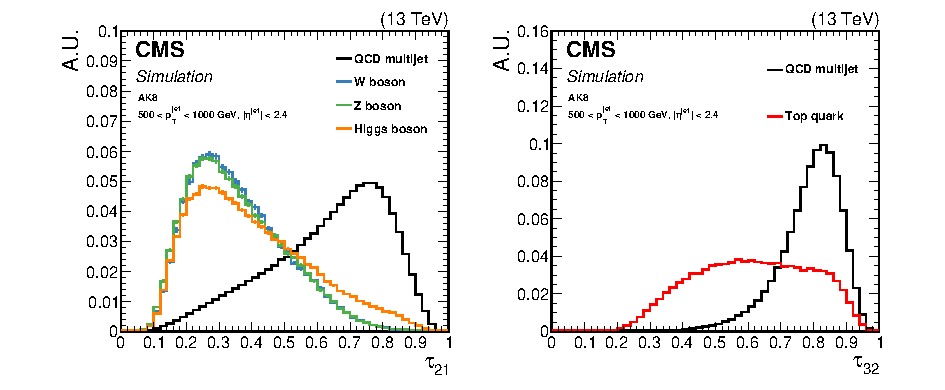
\includegraphics[width=0.9\textwidth]{figures/CMS_JME_18_002_Figure_003.pdf}
  \caption[Comparison of \( \tau_{21} \) and \( \tau_{32} \) shapes for signal and background in AK8 jets]%
  {Comparison of \( \tau_{21} \) and \( \tau_{32} \) shapes for signal and background in AK8 jets.
    The left is \( \tau_{21} \) distribution showing discrimination W/Z/H jets
    vs QCD jet, and the right is \( \tau_{32} \) distribution for t-quark vs
    QCD jets~\cite{cms-jme-deep-tagger}.}%
  \label{fig:cms-tau21-tau32-comparison}
\end{figure}

Deep Tagger for AK8 is a \gls{ML} based tagger developed to determine the
origin of a fatjet. Figure~\ref{fig:cms-deepAK8-arch}
describes the architecture of ``DeepAK8'' tagging. These taggers are trained on particle level information
from \gls{PF}, and provide multi class tagging probabilities such as
\textit{Z} vs. \gls{QCD}, \textit{W} vs. \gls{QCD}, etc.
Since deep taggers utilize deep neutral network with particle level
information their classification power is higher than N-subjetiness,
and are worth the study for future analysis.
%In addition to
%there are version of these taggers is also which is de-correlated from the mass of jet,
%this is important for analysis including this dissertation where we utilize
%mass regions of fatjet to normalize background contribution.

\begin{figure}[!ht]
  \centering
  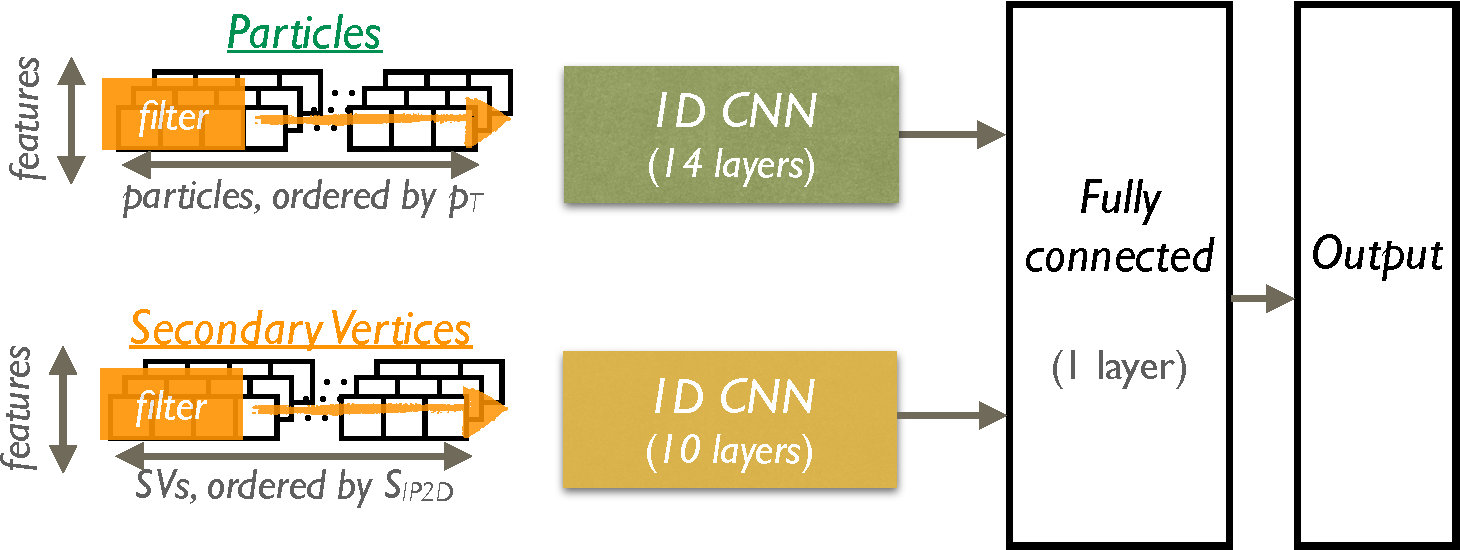
\includegraphics[width=0.7\textwidth]{figures/CMS_JME_18_002_Figure_009.pdf}
  \caption[The network architecture of DeepAK8]%
  {The network architecture of DeepAK8~\cite{cms-jme-deep-tagger}}%
  \label{fig:cms-deepAK8-arch}
\end{figure}

\subsubsection{
  Softdrop Mass
}\label{ch_reco:softdrop}

Fatjets can also have contamination coming from wide angle
soft \gls{ISR} and multiple hadron scattering,
which affects the mass calculation of the jet, to remove
such contamination and have better mass reconstruction, the
``softdrop'' mass algorithm~\cite{softdrop-mass-2014} is used.

Softdrop is a declustering algorithm which removes the particle from the jet
with radius \( R_0 \) (\(=0.8\), for fatjet), when the following condition between two particles is satisfied,
%
\begin{equation}
  \frac{\min(p_{T,1}, p_{T,2})}{p_{T,1} + p_{T,2}} > z_{cut} {\left( \frac{\Delta R_{12}}{R_0} \right)}^{\beta}
\end{equation}

where \( \Delta R_{12} \) is the distance between the two particles, \( z_{cut} \)
and \( \beta \) are the parameters for tuning softdrop declustering.
For fatjets used in \gls{CMS}, the softdrop algorithm is applied with
\( \beta = 0\) and \( z_{cut} = 0.1\) which vetoes both soft
and soft-collinear emissions in a jet.

\subsection{
  Missing transverse momentum
}

Invisible particles like neutrinos cannot be detected at \gls{CMS} directly.
Kinematics of such particles can be determined using the law of conservation of
total momentum. In case of proton-proton collision,
the actual collision happens between quarks contained in
proton which carry an undetermined fraction of proton momentum.
For this reasons kinematic determination
of invisible particles is limited to transverse plane only.

After all the particles are reconstructed in an event, their \( p_T \)'s
can be used to determine missing transverse momentum as,
%
\begin{equation}
  \vec{p}_{T}^{~miss} = - \sum \vec{p}_{T}
\end{equation}

It's usually neutrinos which contributes to missing transverse momentum
and they have very small mass, the missing transverse momentum is then
equivalent to \gls{MET}, which is most often used term in physics analyses.
Experimentally, noise in detector or beam halo of colliding beams
can cause anomalously large missing transverse momentum. There are
various algorithms available in \gls{CMS} that can suppress such events.

\section{
  Monte Carlo (MC) Simulation
 }

In the proton-proton collision, determination of
exact underlying process from reconstructed final state is not possible.
To do measurements on the process of interest,
we need to quantify how much is the signal (process of interest)
and how much is the background (processes with same final state and
similar kinematics). \gls{MC} simulations are employed
to generate underlying processes that can help in the
modeling of signal and background process and compare them against the collision
data.

Main tools and framework
used at \gls{CMS} for generating \gls{MC} events
are described in this section.

\subsection{
  Generators
}

There are three main components to the event generator,
\gls{PDF}, matrix element and parton shower.
\gls{PDF} encodes the probability of finding a patron
with given fraction of energy at given proton momentum.
Matrix element encodes
the theoretical cross-section of the hard process.

Our signal \textit{ZVjj} is a pure \gls{EW} process generated
at \gls{LO} with \MGvATNLO{} and \MADSPIN{}~\cite{madgraph,madspin}.
At \gls{LO} this process has six \gls{EW} vertices, and
zero \texttt{QCD} vertices. The generation is done
in two steps with both vector boson generated on shell
with \MADGRAPH{} and decayed to leptons and quarks via \MADSPIN{}.
For example, to generate \textit{ZZ} process, the syntax used is,

\begin{align*}
   & \texttt{\$ madgraph >}                      \\
   & \texttt{generate p p > z z j j QED=4 QCD=0} \\
   & \texttt{\$ madspin >}                       \\
   & \texttt{decay z > l+ l-}                    \\
   & \texttt{decay z > j j}                      \\
\end{align*}

where \texttt{p} and \texttt{j} are defined as collection of quarks of gluons,
\texttt{z} is the on-shell \textit{Z} boson, and \texttt{l+}, \texttt{l-}
are the leptons consisting of electrons, muons and taus. The syntax
indicates \texttt{QED=4 QCD=0} implies that there are four \gls{EW}
vertices, since we are first generating \textit{Z} on-shell, and zero
\texttt{QCD} vertices. The last two \gls{EW} vertices comes from
decay of \textit{Z} bosons to fermions.

\subsection{
  Parton Shower and Hadronization
}

After events are generated with the hard process of interest,
they go through the process of parton shower and hadronization
to simulate QCD bremsstrahlung radiation
and make final state hadrons to preserve overall color charge of an event.
This is done because quarks and gluons coming from hard process scattering
cannot stay free and produce quark-antiquark pair
or radiate gluons.
The parton shower software simulates this process until partons
have reached low energy of the order of 1 \GeV{}.

After all the partons have showered, they go through the process of
hadronization to produce final state hadrons.
Hadronization is done using the models that are tuned on experimental data.
Most of the models used for \gls{MC} in standard model physics at \gls{CMS}
are based on the Lund string model in the \PYTHIA{} framework~\cite{pythia}.
Most showers are usually collimated and they appear
as jets in the final state, but sometimes a highly energetic gluon
can radiate a high energy gluon which will eventually
make a new jet, it can be either \gls{ISR} during the hard process,
or \gls{FSR} during the parton shower.
This increases jets multiplicity of an event,
since we have four jets in our final state this step is important for
accurate modeling of our background processes.

\subsection{Tunes}

In hadron-hadron collisions there are two additional interactions,
\glspl{BBR} and \glspl{MPI}, they are modeled as \gls{UE}.
\gls{BBR} is what left behind by incoming beam hadron and does
not take part in \gls{ISR} or hard scattering, and these remnants
need to be color connected with the rest of the event.
The \glspl{MPI} are the additional multiple interaction that a parton
can go through in the same hadron-hadron collision,
these interactions can be hard or semi-hard.
To model \gls{UE} properly in standard \gls{MC} event generator,
a set of parameters (referred as ``tune'') are needed
to be adjusted so that it provides better fit to the experiment data.
\gls{CMS} made use of the tune \texttt{TuneCUETP8M1}~\cite{pythia8-tune-CUETP8M1}
(2016 \glspl{MC} samples) and \texttt{TuneCP5}~\cite{pythia8-tune-cp5} (2017 and 2018 \glspl{MC} samples)
in the \PYTHIA{} for modeling \gls{UE}.